\section{Itthipaṇḍaka, Animittā, Nimittamattā, Vepurisikā}

These four terms mentioned in the {\em Bhikkhunikkhandhaka} are rather vague in their descriptions. The Chinese texts are not very clear on this point either but the overall questions asked here seem to have mostly to do with menstruation and diseases. At first glance it seems that the rules regarding ordination are trying to make sure that the girl in question is old enough for ordination and not ill. Rules concerning whether or not a girl has breasts can be explained as a question with regards to age, or it can be explained as a girl who has not developed the secondary characteristics needed i.e. possibly intersex. The question about whether a girl is sterile or barren would point to her at least having had one child but this would seem strange if she wants to enter a celibate order. 

\cite{sujato2009} points out that the Bhikkhunī Vinaya uses its own language and terminology that is often more in line with the Jain terminology and is poorly integrated with the Bhikkhu Vinaya. This could explain the discrepancies we see between the Bhikkhu and Bhikkhunī Vinaya in describing certain words pertaining to gender. In any case, the variabilty and vagueness of these terms with reference to gender do not permit a clear picture.

The following table gives an overview of the terms:

\bigskip
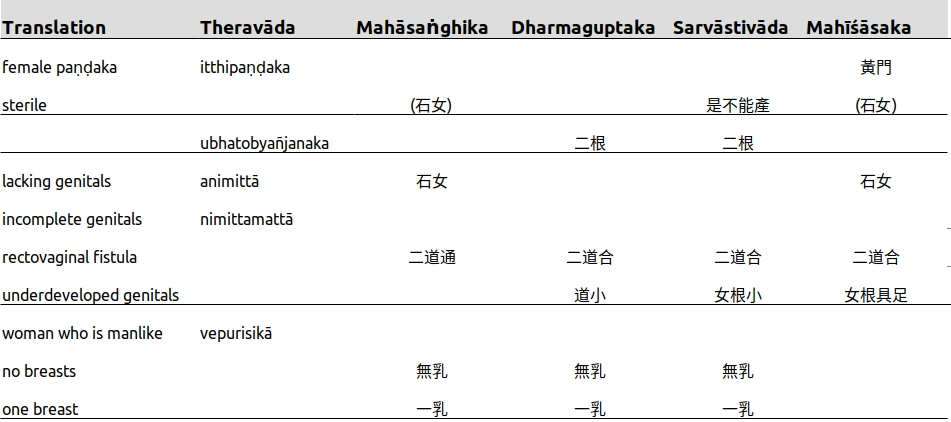
\includegraphics[width=\linewidth]{female.jpg}
\label{female}

It is certain though that the terms of {\em paṇḍaka} and {\em ubhatob­yañ­janaka} pertained primarily to male candidates as we have also seen in the Jain order while the Bhikkhunī seem to have had their own vocabulary.

There are some rare cases of people who are raised from birth as girls that later became assigned as hijra after they failed to develop secondary female sexual characteristics (breast development and menarche) at puberty\footnote{\cite{nanda}}. Although there is very little evidence to go on, I believe that these respresent the {\em itthipaṇḍaka}.

At least in the Bhikkhunī ordination in the Theravāda lineage, the {\em animittā, nimittamattā and vepurisikā} are allowed to ordain. This is possibly also true in several of the Chinese Vinaya.
